\section{port numbers}
\begin{frame}{port numbers}
    \begin{itemize}
    \item we run multiple programs on a machine
        \begin{itemize}
        \item IP addresses identifying machine --- not enough
        \end{itemize}
    \item<2-> so, add 16-bit \textit{port numbers}
        \begin{itemize}
        \item<2-> think: multiple PO boxes at address
        \end{itemize}
    \vspace{.5cm}
    \item<3-> 0--49151: typically assigned for particular services
        \begin{itemize}
        \item 80 = http, 443 = https, 22 = ssh, \ldots
        \item usually <1024 reserved for sysadmin-only-use
        \end{itemize}
    \item<3-> 49152--65535: allocated on demand
        \begin{itemize}
        \item default ``return address'' for client connecting to server
        \end{itemize}
    \end{itemize}
\end{frame}

\begin{frame}{sockets}
    \begin{itemize}
    \item port number helps identify \textit{sockets}
    \item sockets = file applications use to access networks
    \end{itemize}
\end{frame}

\begin{frame}{port number independence}
    \begin{itemize}
    \item typically ``5-tuple'' identifies ``socket'': \\
        (protocol=TCP or UDP, source IP, dest IP, source port, dest port)
    \item means can have:
        \begin{itemize}
        \item two sockets with same source IP+source port, but different destinations
        \item two sockets with same dest IP+des port, but different sources
        \item two sockets with different protocols, but everything else same
        \end{itemize}
    \item special cases:
        \begin{itemize}
        \item dest IP/port can be `wildcard' (all zeroes usually)
        \item used for server that can be connected to
        \item used for unconnected UDP sockets
        \end{itemize}
    \end{itemize}
\end{frame}


\section{UDP}
\usetikzlibrary{patterns.meta}
\begin{frame}[fragile]{UDP format}
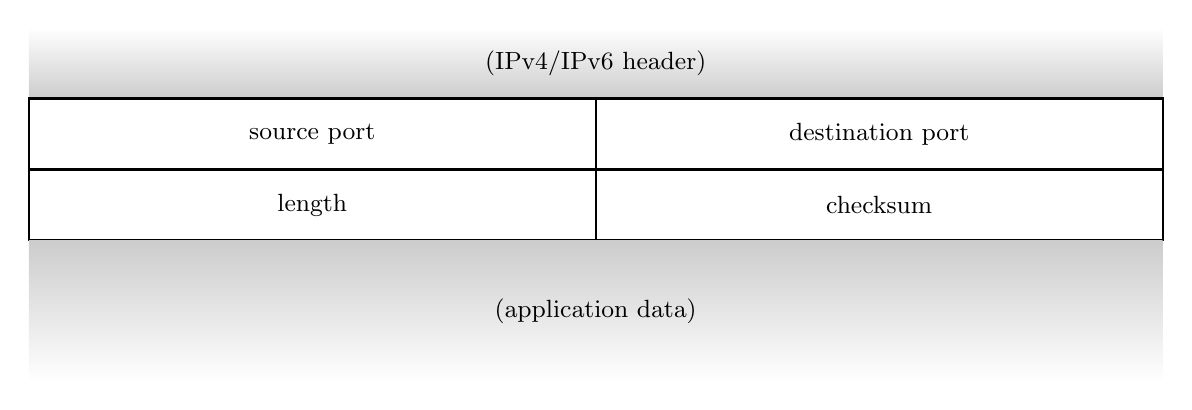
\begin{tikzpicture}
\tikzset{
    box/.style={draw,thick},
    label/.style={font=\small},
    label large/.style={},
    box label/.style={midway,font=\small,align=center},
    box label flags/.style={midway,font=\fontsize{8}{9}\selectfont,align=center},
    missing/.style={pattern=north west lines},
}
\begin{scope}[x=0.45cm,y=0.9cm]
\path[shading=axis,top color=white,bottom color=black!20] (0, 1) rectangle (32, 0)
    node[box label] {(IPv4/IPv6 header)};
\draw[box] (0, 0) rectangle (16, -1)
    node[midway,label] {source port};
\draw[box] (16, 0) rectangle (32, -1)
    node[midway,label] {destination port };
\draw[box] (0, -1) rectangle (16, -2)
    node[midway,label] {length};
\draw[box] (16, -1) rectangle (32, -2)
    node[midway,label] {checksum};
\path[shading=axis,bottom color=white,top color=black!20] (0, -2) rectangle (32, -4)
    node[box label] {(application data)};
\end{scope}
\end{tikzpicture}
\end{frame}


\section{BSD socket history}
\begin{frame}{BSD sockets}
    \begin{itemize}
    \item BSD = Berkely Standard Distribution (of Unix)
    \item interface designed for stream connections
    \item current C version standardized by POSIX
    \item pretty much default interface programming with TCP connections
        \begin{itemize}
        \item \ldots across all platforms
        \end{itemize}
    \end{itemize}
\end{frame}


\section{UDP sockets}
\begin{frame}[fragile]{unconnected UDP sockets (Python)}
\begin{Verbatim}[fontsize=\small]
import socket
# ipv4
sock = socket.socket(socket.AF_INET, socket.SOCK_DGRAM)
sock = socket.socket(socket.AF_INET, socket.SOCK_DGRAM,
                     socket.IPPROTO_UDP)
# ipv6
sock = socket.socket(socket.AF_INET6, socket.SOCK_DGRAM)
sock = socket.socket(socket.AF_INET6, socket.SOCK_DGRAM,
                     socket.IPPROTO_UDP)

sock.bind((local_host, local_port))
# local_host == "0.0.0.0" (v4) or "::" (v6) for "all possible"

data1, (host1, port1) = sock.recvfrom(MAX_SIZE)
sock.sendto(data, (host2, port2))
\end{Verbatim}
\end{frame}

\begin{frame}[fragile]{unconnected UDP sockets (Python, generic)}
\begin{Verbatim}[fontsize=\fontsize{9}{10}\selectfont]
import socket
possible_local_addrs = socket.getaddrinfo(
        local_host, local_port,
        family=socket.AF_UNSPEC,
        type=socket.SOCK_DGRAM,
        flags=socket.AI_PASSIVE)

for af, socktype, proto, canonname, sockaddr in possible_local_addrs:
    sock = socket.socket(af, socktype, proto)
    sock.bind(sockaddr)
    # then use sock for recvfrom/sendto somehow
\end{Verbatim}
\end{frame}

\begin{frame}[fragile]{unconnected UDP sockets (Python, generic)}
\begin{Verbatim}[fontsize=\fontsize{9}{10}\selectfont]
import socket
possible_remote_addrs = socket.getaddrinfo(
        remote_host, remote_port,
        family=socket.AF_UNSPEC,
        type=socket.SOCK_DGRAM,
        flags=0)

for af, socktype, proto, canonname, sockaddr in possible_remote_addrs:
    sock = socket.socket(af, socktype, proto)
    try:
        # hope local_host is acceptable for 'af'?
        # maybe choose local_host based on 'af' value?
        sock.bind((local_host, local_addr))
        sock.sendto(data, ...)
        ...
    except ...:
        ...
        # hope another address works?
        continue
\end{Verbatim}
\end{frame}

\begin{frame}{aside: getaddrinfo}
    \begin{itemize}
    \item lookup host+port by name
    \item can handle both IPv4 and IPv6
    \item AI\_PASSIVE = for bind()
    \item returns list of addresses
        \begin{itemize}
        \item sometimes: just choose one address (send message to server)
        \item sometimes: want to make socket for each address (run server)
        \end{itemize}
    \end{itemize}
\end{frame}

\begin{frame}[fragile]{unconnected UDP sockets (C, IPv4)}
\begin{Verbatim}[fontsize=\fontsize{9}{10}\selectfont]
int fd = socket(AF_INET, SOCK_DGRAM, 0 /* or IPPROTO_UDP */);
/* for 10.1.2.3 port 12345 
   there are utility functions to help with this, so you 
   shouldn't actually construct local_addr manually like this */
struct sockaddr_in local_addr;
memset(&local_addr, 0, sizeof(local_addr);
local_addr.sin_family = AF_INET;
local_addr.sin_port = htons(12345);
local_addr.sin_addr.s_addr = htonl((10<<24)|(1<<16)|(2<<8)|3),
bind(fd, &local_addr, sizeof(local_addr));
struct sockaddr_in remote1, remote2;
recvfrom(fd, buffer1, buffer1_size, 0, &remote1, sizeof(remote1));
recvfrom(fd, buffer2, buffer2_size, 0, &remote2, sizeof(remote2));
struct sockaddr_in remote3 = ...;
sendto(fd, buffer3, buffer3_size, 0, &remote3, sizeof(remote3));
\end{Verbatim}
\end{frame}

\begin{frame}[fragile]{connected UDP sockets (Python)}
\begin{Verbatim}[fontsize=\small]
import socket
# ipv4
sock = socket.socket(socket.AF_INET, socket.SOCK_DGRAM)
# ipv6
sock = socket.socket(socket.AF_INET6, socket.SOCK_DGRAM)

sock.bind((local_host, local_port))
sock.connect((remote_host, remote_port))
sock.send(b"one datagram")
sock.send(b"another datagram")
remote_data1 = sock.recv(MAX_SIZE)
remote_data2 = sock.recv(MAX_SIZE)
\end{Verbatim}
\end{frame}

\begin{frame}{choosing v4/v6?}
    \begin{itemize}
    \item nicer to write applications that handle both
    \item \ldots without explicitly doing this differently
    \vspace{.5cm}
    \item later socket API for that is getaddrinfo()
        \begin{itemize}
        \item also exists in C, but lots of extra stuff to handle types, etc.
        \end{itemize}
    \end{itemize}
\end{frame}


% FIXME: rearrange to put UDP sockets first, then talk about TCP

\subsection{netstat (UDP)}
\begin{frame}[fragile]{netstat}
\begin{Verbatim}[fontsize=\fontsize{9}{10}]
$ netstat --udp -na
Active Internet connections (servers and established)
Proto Recv-Q Send-Q Local Address           Foreign Address         State      
udp        0      0 128.143.71.27:60001     0.0.0.0:*                          
udp        0      0 128.143.71.27:60002     0.0.0.0:*                          
udp        0      0 128.143.71.27:60003     0.0.0.0:*                          
...
udp        0      0 128.143.71.27:68        128.143.67.64:67        ESTABLISHED
...
udp        0      0 127.0.0.1:123           0.0.0.0:*                          
udp        0      0 0.0.0.0:38269           0.0.0.0:*                          
udp        0      0 0.0.0.0:55407           0.0.0.0:*                          
udp        0      0 0.0.0.0:55786           0.0.0.0:*                          
...
udp6       0      0 :::45631                :::*                               
udp6       0      0 :::111                  :::*                               
udp6       0      0 fe80::1a66:daff:fe2:123 :::*                               
...
\end{Verbatim}
\end{frame}


\section{TCP client sockets}
\begin{frame}[fragile,label=connSetupClientAddrInfo]{connection setup: client, TCP+IPv4}
\begin{lstlisting}[
    language=Python,style=smaller,
    moredelim={**[is][\btHL<2|handout:2>]{@2}{2@}},
    moredelim={**[is][\btHL<3|handout:3>]{@3}{3@}},
    moredelim={**[is][\btHL<4|handout:4>]{@4}{4@}},
    moredelim={**[is][\btHL<5|handout:5>]{@5}{5@}},
    moredelim={**[is][\btHL<6|handout:6>]{@6}{6@}},
]
sock = socket.socket(socket.AF_INET, socket.SOCK_STREAM)
# to select local host/port: socket.bind(('128.143.71.27', 54444))
# if no local host/port selected, OS assigns
sock.connect(('128.143.67.8', 443))
...
sock.send(...)
sock.recv(...)
\end{lstlisting}
\end{frame}

\begin{frame}[fragile,label=connSetupClientAddrInfo]{connection setup: client, TCP+IPv6}
\begin{lstlisting}[
    language=Python,style=smaller,
    moredelim={**[is][\btHL<2|handout:2>]{@2}{2@}},
    moredelim={**[is][\btHL<3|handout:3>]{@3}{3@}},
    moredelim={**[is][\btHL<4|handout:4>]{@4}{4@}},
    moredelim={**[is][\btHL<5|handout:5>]{@5}{5@}},
    moredelim={**[is][\btHL<6|handout:6>]{@6}{6@}},
]
sock = socket.socket(socket.AF_INET6, socket.SOCK_STREAM)
# to select local host/port: socket.bind(('3fff:1234::1', 54444))
# if no local host/port selected, OS assigns
sock.connect(('2607:f8b0:4004:c06::67', 443))
...
sock.send(...)
sock.recv(...)
\end{lstlisting}
\end{frame}


\begin{frame}[fragile,label=connSetupClientAddrInfo]{connection setup: generic TCP, addrinfo}
\begin{Verbatim}[fontsize=\fontsize{9}{10}]
import socket
possible_addrs = socket.getaddrinfo(
        'www.cs.virginia.edu', '443',
        socket.AF_UNSPEC, socket.SOCK_STREAM)

for af, socktype, proto, canonname, sockaddr in possible_addrs:
    try:
        sock = socket.socket(af, socktype, proto)
    except OSError:
        sock = None
        continue
    try:
        sock.connect(sa)
    except OSError:
        sock.close()
        sock = None
        continue

if sock == None:
    # not successful
\end{Verbatim}
\end{frame}

 

\subsection{partial/split read/writes}
\usetikzlibrary{arrows.meta}
\begin{frame}{size mismatch? (1)}
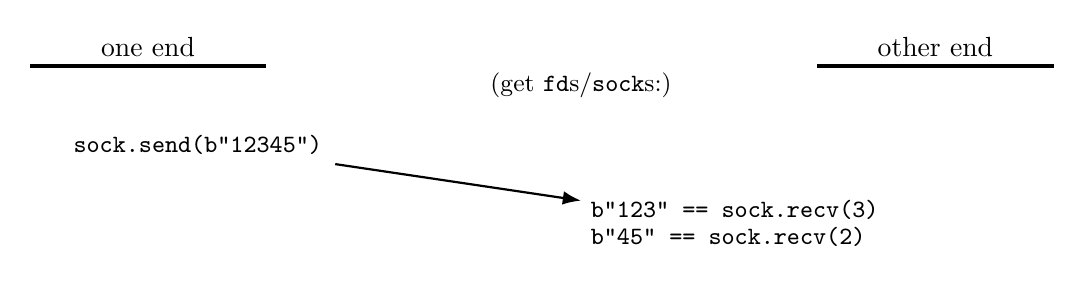
\begin{tikzpicture}
\tikzset{>=Latex}
\node[anchor=south] at (1.5, 0) {one end};
\draw[ultra thick] (0, 0) -- ++(3, 0);
\draw[ultra thick] (10, 0) -- ++(3, 0);
\node[anchor=south] at (11.5, 0) {other end};
\node[font=\small] at (7, -.25) {(get \texttt{fd}s/\texttt{sock}s:)};
\tikzset{
    function/.style={font=\fontsize{9}{10}\tt\selectfont,align=left},
}
\node[function,anchor=east] (write 1) at (4, -1) {
sock.send(b"12345")
};
\node[function,anchor=west] (read 1) at (7, -2) {
b"123" == sock.recv(3) \\
b"45" == sock.recv(2) 
};
\draw[thick,->] (write 1) -- (read 1);
\end{tikzpicture}
\end{frame}

\begin{frame}{size mismatch? (2)}
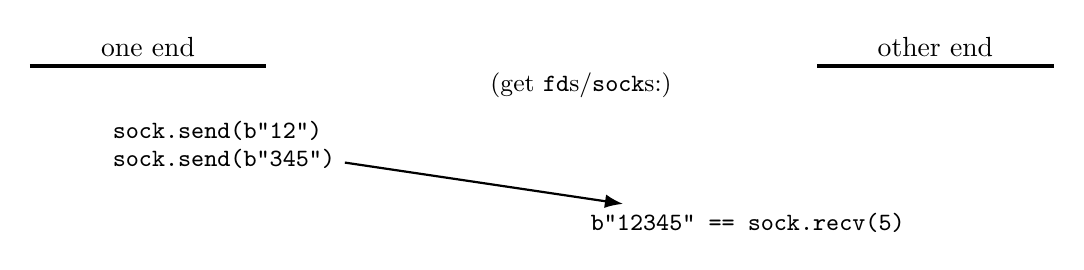
\begin{tikzpicture}
\tikzset{>=Latex}
\node[anchor=south] at (1.5, 0) {one end};
\draw[ultra thick] (0, 0) -- ++(3, 0);
\draw[ultra thick] (10, 0) -- ++(3, 0);
\node[anchor=south] at (11.5, 0) {other end};
\node[font=\small] at (7, -.25) {(get \texttt{fd}s/\texttt{sock}s:)};
\tikzset{
    function/.style={font=\fontsize{9}{10}\tt\selectfont,align=left},
}
\node[function,anchor=east] (write 1) at (4, -1) {
sock.send(b"12") \\
sock.send(b"345")
};
\node[function,anchor=west] (read 1) at (7, -2) {
b"12345" == sock.recv(5)
};
\draw[thick,->] (write 1) -- (read 1);
\end{tikzpicture}
\end{frame}

\begin{frame}{partial reads?}
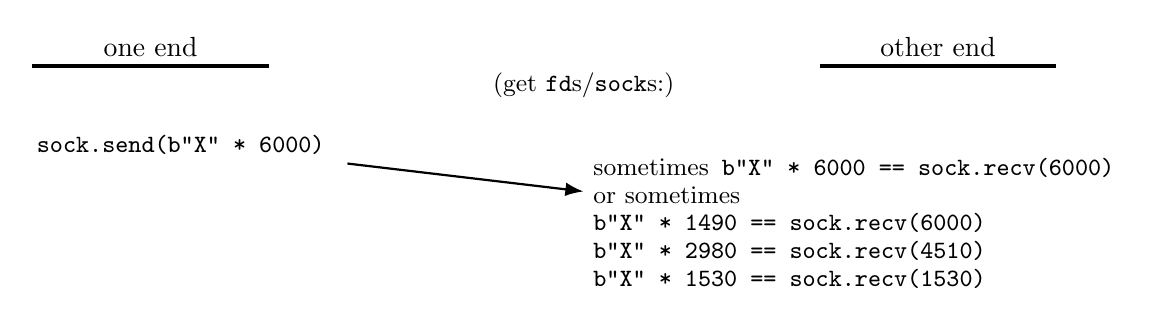
\begin{tikzpicture}
\tikzset{>=Latex}
\node[anchor=south] at (1.5, 0) {one end};
\draw[ultra thick] (0, 0) -- ++(3, 0);
\draw[ultra thick] (10, 0) -- ++(3, 0);
\node[anchor=south] at (11.5, 0) {other end};
\node[font=\small] at (7, -.25) {(get \texttt{fd}s/\texttt{sock}s:)};
\tikzset{
    function/.style={font=\fontsize{9}{10}\tt\selectfont,align=left},
}
\node[function,anchor=east] (write 1) at (4, -1) {
sock.send(b"X" * 6000)
};
\node[function,anchor=west] (read 1) at (7, -2) {
\textit{\normalfont sometimes} b"X" * 6000 == sock.recv(6000) \\
\textit{\normalfont or sometimes} \\
b"X" * 1490 == sock.recv(6000) \\
b"X" * 2980 == sock.recv(4510) \\
b"X" * 1530 == sock.recv(1530) 
};
\draw[thick,->] (write 1) -- (read 1);
\end{tikzpicture}
\end{frame}

\begin{frame}{partial writes}
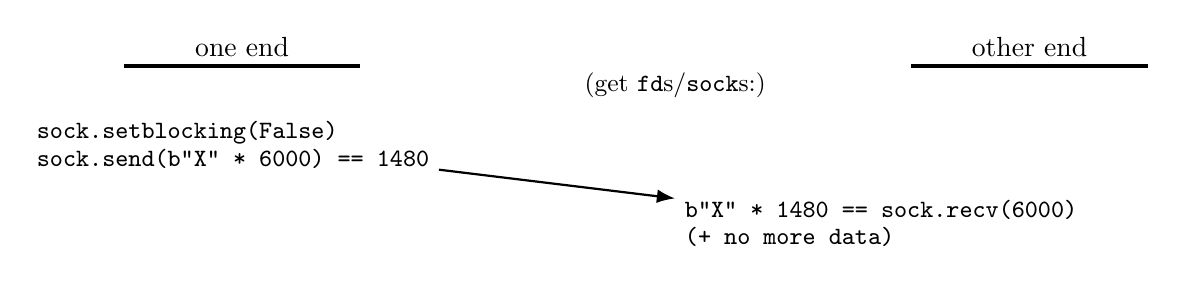
\begin{tikzpicture}
\tikzset{>=Latex}
\node[anchor=south] at (1.5, 0) {one end};
\draw[ultra thick] (0, 0) -- ++(3, 0);
\draw[ultra thick] (10, 0) -- ++(3, 0);
\node[anchor=south] at (11.5, 0) {other end};
\node[font=\small] at (7, -.25) {(get \texttt{fd}s/\texttt{sock}s:)};
\tikzset{
    function/.style={font=\fontsize{9}{10}\tt\selectfont,align=left},
}
\node[function,anchor=east] (write 1) at (4, -1) {
sock.setblocking(False) \\
sock.send(b"X" * 6000) == 1480
};
\node[function,anchor=west] (read 1) at (7, -2) {
b"X" * 1480 == sock.recv(6000) \\
(+ no more data)
};
\draw[thick,->] (write 1) -- (read 1);
\end{tikzpicture}
\end{frame}

\begin{frame}{partial reads/writes}
    \begin{itemize}
    \item read/recv can have read less than requested
        \begin{itemize}
        \item read of zero bytes = end of file
        \end{itemize}
    \item send/write can write less than requested\ldots \\
        but only on error or if non-blocking mode requested
    \end{itemize}
\end{frame}

\begin{frame}{incomplete writes}
\begin{itemize}
    \item \texttt{send} might write less than requested
        \begin{itemize}
        \item error after writing some data
        \item if blocking disabled
        \end{itemize}
    \item \texttt{recv} might read less than requested
        \begin{itemize}
        \item error after reading some data
        \item not enough data got there in time
        \end{itemize}
\end{itemize}
\end{frame}


\subsection{simultaneous read/write}
\begin{frame}{reading and writing at once}
    \begin{itemize}
    \item so far assumption: alternate between reading+writing
        \begin{itemize}
        \item sufficient for FTP assignment
        \item how many protocols work
        \end{itemize}
    \item ``half-duplex''
    \item don't have to use sockets this way, but tricky
        \vspace{.5cm}
    \item threads: one reading thread, one writing thread \textit{OR}
    \item event-loop: use \textit{non-blocking I/O} and select()/poll()/etc. functions
        \begin{itemize}
        \item non-blocking I/O setup with fcntl() function
        \item non-blocking write() fills up buffer as much as possible, then returns
        \item non-blocking read() returns what's in buffer, never waits for more
        \end{itemize}
    \end{itemize}
\end{frame}


\section{TCP server sockets}
\subsection{server socket idea}
\usetikzlibrary{arrows.meta,calc}


\begin{frame}{sockets and server sockets (C)}
% FIXME
\begin{tikzpicture}
    \tikzset{
        >=Latex,
        comp box/.style={draw, thick, align=center, minimum width=1.5cm,minimum height=1.5cm},
        explain box/.style={draw=red,very thick, align=left},
        msg/.style={font=\small},
        cmd/.style={font=\small},
    }
    \node[draw,circle,label={south:client}] (client) {socket};
    \node[draw,circle,align=center] (ssocket) at ([xshift=8.75cm,yshift=4cm]client.west) {server\\socket};
    \node[draw,circle,align=center,label={south:server},visible on=<4->] (server) at ([xshift=8.75cm]client.west) {socket};
    \draw[very thick,dotted,<-] (ssocket.east) -- ++(.5cm,0cm) node[right,font=\small\tt,align=left] {
        server: \\
        \myemph<2>{ss\_fd = socket(\ldots)} \\
        \myemph<3>{bind(ss\_fd, addr, \ldots)} \\
        \myemph<3>{listen(ss\_fd, \ldots)}
    };
    \draw[very thick,dotted,<-] (client.north) -- ++(0cm,2cm) node[above,xshift=1cm,font=\small\tt,align=left] {
        client: \\
        \myemph<2>{fd = socket(\ldots)}
    };
    \begin{visibleenv}<2>
        \node[explain box,anchor=north] at ([yshift=-.5cm]ssocket.south) {
            socket() function --- create socket fd
        };
    \end{visibleenv}
    \begin{visibleenv}<3>
        \node[explain box,anchor=north] at ([yshift=-.5cm]ssocket.south) {
            listen() --- turn socket into server socket \\
            still has a file descriptor, but \ldots \\
            can only \texttt{accept()} --- create normal socket
        };
    \end{visibleenv}
    \begin{visibleenv}<4->
    \draw[very thick,dotted,->] (client) -- (ssocket)
        node[font=\small,midway,sloped,above,align=left] {request connection \\
                                   client: \texttt{\myemph<4-5>{connect(fd, addr, \ldots)}}};
    \draw[very thick,dotted,->,out=-120,in=120] (ssocket) to (server);
    \node[anchor=west,align=left] at ([xshift=-.75cm]$(server)!0.5!(ssocket)$) {server: \\ \texttt{fd = \myemph<4-5>{accept(ss\_fd, \ldots)}}};
    \end{visibleenv}
    \begin{visibleenv}<5->
    \draw[<->,double,ultra thick] (client) -- (server) node[midway,fill=white,inner sep=0.1mm] {connection};
    \end{visibleenv}
\end{tikzpicture}
\end{frame}


\begin{frame}{sockets and server sockets (Python)}
% FIXME
\begin{tikzpicture}
    \tikzset{
        >=Latex,
        comp box/.style={draw, thick, align=center, minimum width=1.5cm,minimum height=1.5cm},
        explain box/.style={draw=red,very thick, align=left},
        msg/.style={font=\small},
        cmd/.style={font=\small},
    }
    \node[draw,circle,label={south:client}] (client) {socket};
    \node[draw,circle,align=center] (ssocket) at ([xshift=7.75cm,yshift=4cm]client.west) {server\\socket};
    \node[draw,circle,align=center,label={south:server},visible on=<4->] (server) at ([xshift=8.75cm]client.west) {socket};
    \draw[very thick,dotted,<-] (ssocket.east) -- ++(.5cm,0cm) node[right,font=\small\tt,align=left] {
        server: \\
        \myemph<2>{ssock = \textbackslash} \\
        \myemph<2>{\hspace{.25cm}socket.socket(\ldots)} \\
        \myemph<3>{ssock.bind(\ldots)} \\
        \myemph<3>{ssock.listen()}
    };
    \draw[very thick,dotted,<-] (client.north) -- ++(0cm,2cm) node[above,xshift=1cm,font=\small\tt,align=left] {
        client: \\
        \myemph<2>{sock = socket.socket(\ldots)}
    };
    \begin{visibleenv}<2>
        \node[explain box,anchor=north] at ([yshift=-.5cm]ssocket.south) {
            socket() function --- create socket fd
        };
    \end{visibleenv}
    \begin{visibleenv}<3>
        \node[explain box,anchor=north] at ([yshift=-.5cm]ssocket.south) {
            listen() --- turn socket into server socket \\
            still has a file descriptor, but \ldots \\
            can only \texttt{accept()} --- create normal socket
        };
    \end{visibleenv}
    \begin{visibleenv}<4->
    \draw[very thick,dotted,->] (client) -- (ssocket)
        node[font=\small,midway,sloped,above,align=left] {request connection \\
                                   client: \texttt{\myemph<4-5>{sock.connect(\ldots)}}};
    \draw[very thick,dotted,->,out=-120,in=120] (ssocket) to (server);
    \node[anchor=west,align=left] at ([xshift=-.75cm]$(server)!0.5!(ssocket)$) {server: \\ \texttt{sock, addr = \textbackslash} \\ \hspace{.25cm}\myemph<4-5>{\texttt{ssock.accept(\ldots)}}};
    \end{visibleenv}
    \begin{visibleenv}<5->
    \draw[<->,double,ultra thick] (client) -- (server) node[midway,fill=white,inner sep=0.1mm] {connection};
    \end{visibleenv}
\end{tikzpicture}
\end{frame}



\subsection{TCP server setup}
\begin{frame}[fragile]{connection setup: server, IPv4}
\begin{Verbatim}[fontsize=\small]
import socket
ssock = socket.socket(socket.AF_INET, socket.SOCK_STREAM)
# 0.0.0.0 == "any IP address"
ssock.bind(('0.0.0.0', 12345))
ssock.listen()
sock, remote_addr = ssock.accept()
Use(sock)
\end{Verbatim}
\end{frame}

\begin{frame}[fragile]{connection setup: server, IPv4}
\begin{Verbatim}[fontsize=\small]
import socket
ssock = socket.socket(socket.AF_INET, socket.SOCK_STREAM)
# 0.0.0.0 == "any IP address"
ssock.bind(('0.0.0.0', 12345))
ssock.listen()
sock, remote_addr = ssock.accept()
Use(sock)
\end{Verbatim}
\end{frame}

\begin{frame}[fragile,label=connSetupServerLookup]{connection setup: server, generic}
\begin{Verbatim}[fontsize=\fontsize{9}{10}]
import select
import socket
all_addrs = socket.getaddrinfo(
        None, '12345',
        socket.AF_UNSPEC, socket.SOCK_STREAM)
ssocks = []
for af, socktype, proto, canonname, sockaddr in possible_addrs:
    ssock = socket.socket(af, socktype, proto)
    try:
        ssock.bind(sockaddr)
        ssock.listen()
        ssocks.append(ssock)
    except OSError:
        pass

which_ready, _, _ = select.select(ssocks, [], [])
for item in which_ready:
    sock, remote_addr = which_ready.accept()
    Use(sock)
\end{Verbatim}
\end{frame}



\section{connection internals/socket tracking}
\subsection{TCP handshake}
\begin{frame}{three-way TCP handshake}
\begin{tabular}{l@{$\rightarrow$}l|llll}
from & to & flags & seq & ack & data\\
client & server & SYN & $X$ & --- & ---\\
server & client & SYN+ACK & $Y$ & $X+1$ & ---\\
client & server & ACK & $X+1$ & $Y+1$ & ---\\
client & server & ACK & $X+1$ & $Y+1$ & initial data  \\
\end{tabular}
$X$, $Y$ selected at random
\end{frame}

\begin{frame}
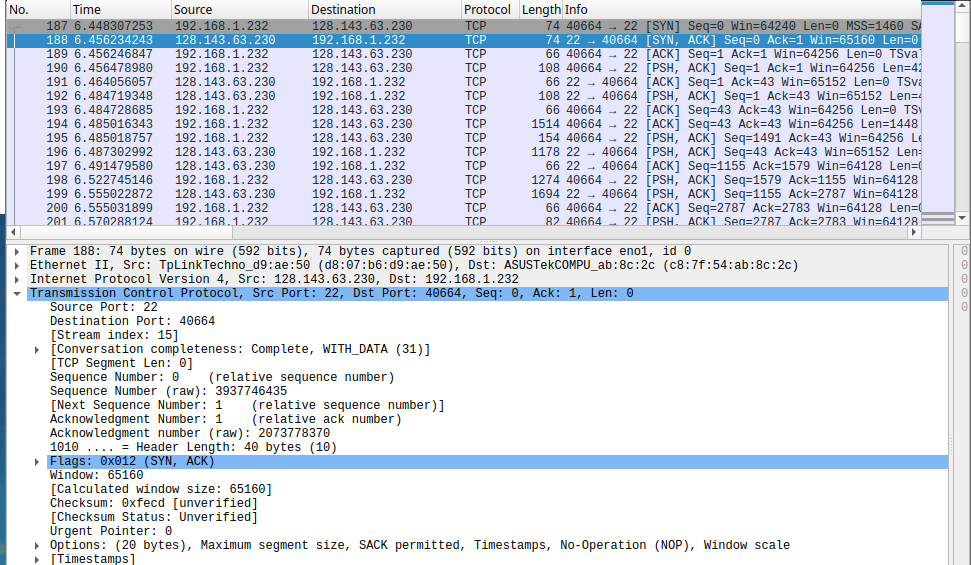
\includegraphics[width=\textwidth]{../sockets/tcp-handshake-wireshark}
\end{frame}

\begin{frame}[fragile]{so many messages?}
    \begin{itemize}
    \item TCP waits full round-trip before sending data; can do better
    \item example: QUIC (figure from RFC 9000, TCP+TLS replacement)
    \end{itemize}
\begin{Verbatim}[fontsize=\fontsize{8}{9}\selectfont]
Client                                                  Server

Initial[0]: CRYPTO[CH]
0-RTT[0]: STREAM[0, "..."] ->

                                 Initial[0]: CRYPTO[SH] ACK[0]
                                  Handshake[0] CRYPTO[EE, FIN]
                          <- 1-RTT[0]: STREAM[1, "..."] ACK[0]

Initial[1]: ACK[0]
Handshake[0]: CRYPTO[FIN], ACK[0]
1-RTT[1]: STREAM[0, "..."] ACK[0] ->

                                          Handshake[1]: ACK[0]
         <- 1-RTT[1]: HANDSHAKE_DONE, STREAM[3, "..."], ACK[1]

Figure 6: Example 0-RTT Handshake
\end{Verbatim}
\end{frame}


\subsection{TCP state machine}
\begin{frame}{TCP state machine}
\begin{tikzpicture}
\node (state) {
    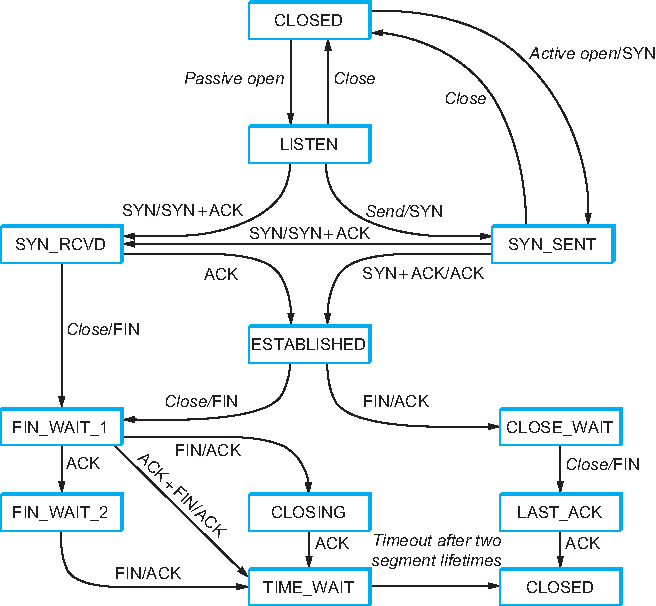
\includegraphics[height=0.8\textheight]{../sockets/sysapproach-tcp-state-fig}
};
\node[anchor=north west] at (state.north east) {
   notation: event/action  \\
   ~ \\
   not shown explicitly: timeout/resend
};
\end{tikzpicture}
\end{frame}


\begin{frame}{connection close}
    \begin{itemize}
    \item FIN (I want to close) + ACK (confirm close)
    \vspace{.5cm}
    \item ACK side needs to wait just in case FIN resent
        \begin{itemize}
        \item keep port number from being reused
        \item TIME\_WAIT state
        \end{itemize}
    \end{itemize}
\end{frame}

\begin{frame}{RST}
    \begin{itemize}
    \item RST (reset) flag often used to respond to unexpected packets
    \item example: data packet for never-established connection
    \end{itemize}
\end{frame}


\subsection{netstat (TCP)}

\begin{frame}[fragile,label=laptopNetstat]{connections on my desktop}
\begin{lstlisting}[language={},basicstyle=\fontsize{9.5}{10.5}\selectfont]
cr4bd@reiss-t3620
: /zf14/cr4bd ; netstat --inet --inet6 --numeric
Active Internet connections (w/o servers)
Proto Recv-Q Send-Q Local Address           Foreign Address         State      
tcp        0      0 128.143.67.91:49202     128.143.63.34:22        ESTABLISHED
tcp        0      0 128.143.67.91:803       128.143.67.236:2049     ESTABLISHED
tcp        0      0 128.143.67.91:50292     128.143.67.226:22       TIME_WAIT  
tcp        0      0 128.143.67.91:54722     128.143.67.236:2049     TIME_WAIT  
tcp        0      0 128.143.67.91:52002     128.143.67.236:111      TIME_WAIT  
tcp        0      0 128.143.67.91:732       128.143.67.236:63439    TIME_WAIT  
tcp        0      0 128.143.67.91:40664     128.143.67.236:2049     TIME_WAIT  
tcp        0      0 128.143.67.91:54098     128.143.67.236:111      TIME_WAIT  
tcp        0      0 128.143.67.91:49302     128.143.67.236:63439    TIME_WAIT  
tcp        0      0 128.143.67.91:50236     128.143.67.236:111      TIME_WAIT  
tcp        0      0 128.143.67.91:22        172.27.98.20:49566      ESTABLISHED
tcp        0      0 128.143.67.91:51000     128.143.67.236:111      TIME_WAIT  
tcp        0      0 127.0.0.1:50438         127.0.0.1:631           ESTABLISHED
tcp        0      0 127.0.0.1:631           127.0.0.1:50438         ESTABLISHED
\end{lstlisting}
\end{frame}
% FIXME: flow chart




\section{more socket customization}
\subsection{setsockopt}
\begin{frame}[fragile]{socket options}
\begin{itemize}
\item `socket options' for extra settings
\item Python: \texttt{sock.setsockopt(level, key, value)}
\item C: \texttt{setsockopt(sock, level, key, value)}
\vspace{.5cm}
\item common level values
    \begin{itemize}
    \item \texttt{SOL\_SOCKET} --- OS-level
    \item \texttt{IPPROTO\_IP}
    \item \texttt{IPPROTO\_IPV4}
    \item \texttt{IPPROTO\_TCP}
    \end{itemize}
\end{itemize}
\end{frame}

\begin{frame}{common SOL\_SOCKET options}
    \begin{itemize}
    \item \texttt{SO\_REUSEADDR} --- allow bind()ing even if another socket for this port active
        \begin{itemize}
        \item common problem: server can't bind() because old session in TIME\_WAIT
        \end{itemize}
    \item \texttt{SO\_RCVBUF} --- buffer size used by OS for receiving bytes
    \item \texttt{SO\_SNDBUF} --- buffer size used by OS for sending bytes
    \vspace{.5cm}
    \item (full list on Linux: \texttt{man 7 socket})
    \end{itemize}
\end{frame}



\subsection{Nagle, etc.}
\begin{frame}[fragile]{efficiency problem}
\begin{Verbatim}[fontsize=\small]
sock = ...
sock.send(b'About to send file with 16Kbytes')
sock.send(b'File is HTML; updated 16 November')
sock.send(file_data)
\end{Verbatim}
\begin{itemize}
\item Naive approach:
    \begin{itemize}
    \item one packet for `about to send file with\ldots'
    \item one packet for `file is HTML; \ldots'
    \item some number of packets for \texttt{file\_data}
    \end{itemize}
\item sending small TCP packets, so lots of overhead
\end{itemize}
\end{frame}

\begin{frame}{Nagle's algorithm}
\begin{itemize}
\item (RFC 896)
\item delay sending data when smaller than full TCP segment
\item hope: by waiting we'll get a full TCP segment
    \begin{itemize}
    \item typical wait: 200 ms?
    \end{itemize}
\vspace{.5cm}
\item TCP\_NODELAY socket option can disable (at least on Linux)
\end{itemize}
\end{frame}


\subsubsection{broadcast}
\begin{frame}{broadcast/multicast}
\begin{itemize}
\item IPv4: can broadcast to every machine on local network
    \begin{itemize}
    \item set the SO\_BROADCAST socket option to 1
    \item send to special address 255.255.255.255 
    \item received at that port number on all machines
    \end{itemize}
\item multicast (send-to-many) groups
    \begin{itemize}
    \item request to receive: IP\_ADD\_MEMBERSHIP (v4), IPV6\_ADD\_MEMBERSHIP (v6)
    \item each `multicast group' has IP address
    \item 224.0.0.0/24 and ff02::/16 = local network only
    \item local network version usually implemented by broadcasting + filtering by IP
    \item (non-local-network multicast is more complex\ldots)
    \end{itemize}
\end{itemize}
\end{frame}

\begin{frame}{service discovery}
\begin{itemize}
\item example: find printers on local network automatically
\vspace{.5cm}
\item typical protocol mDNS (`multicast DNS')
\item uses IP addressses 224.0.0.251 / ff02::fb + port 5353
\item all machines on local network receive from all other machines on local network
\end{itemize}
\end{frame}


\section{aside: other address families}
\begin{frame}{other address families}
    \begin{itemize}
    \item AF\_UNIX {\small (= AF\_LOCAL in C, but not Python)}
        \begin{itemize}
        \item sockets can be represented in files on disk
        \item support sending file descriptors usually
        \end{itemize}
    \item (not sure how portable?) AF\_RAW
        \begin{itemize}
        \item usually how wireshark captures packets on Linux
        \item also supports writing packets
        \end{itemize}
    \item (Linux only) AF\_NETLINK 
        \begin{itemize}
        \item communicate with kernel networking code
        \end{itemize}
    \item AF\_AX25, AF\_APPLETALK, AF\_DECNET, \ldots
        \begin{itemize}
        \item other interesting protocols
        \end{itemize}
    \end{itemize}
\end{frame}

